% https://tex.stackexchange.com/a/313363
\documentclass{beamer}

\usepackage{tikz}
\usetikzlibrary{mindmap}

\tikzset{level 1 concept/.append style={font=\sf, sibling angle=72,level distance = 35mm}}
\tikzset{level 2 concept/.append style={font=\sf, sibling angle=45,level distance = 20mm}}
\tikzset{level 3 concept/.append style={font=\sf, sibling angle=45,level distance = 20mm}}

\begin{document}

    \begin{frame}
        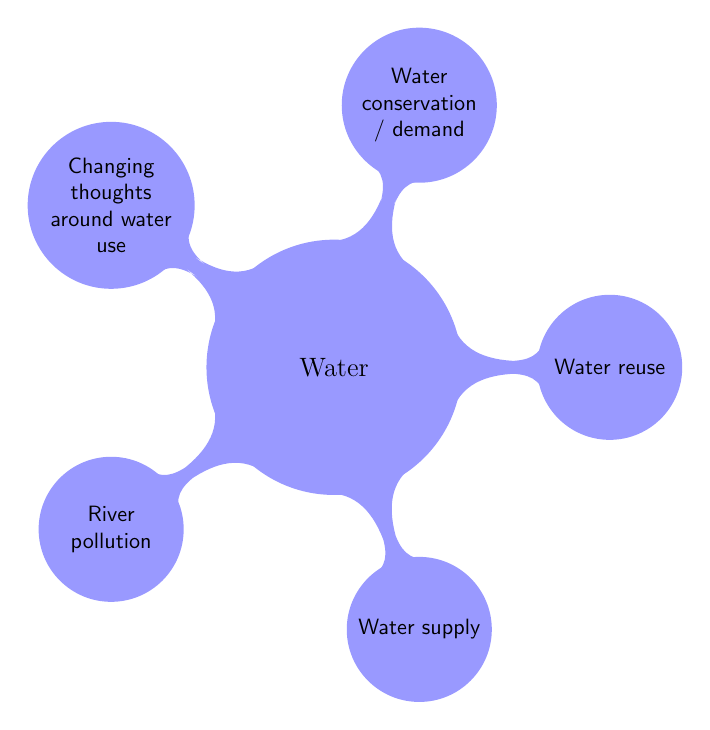
\begin{tikzpicture}[mindmap, grow cyclic, every node/.style=concept, concept color=blue!40, align=flush center]
        \node[scale=0.8]{Water}
        child { node[scale=0.8] {River pollution}}
        child { node[scale=0.8] {Water supply}}
        child { node[scale=0.8] {Water reuse}}
        child { node[scale=0.8] {Water conservation / demand}}
        child { node[scale=0.8] {Changing thoughts around water use}}
        ;
        \end{tikzpicture}
    \end{frame}

\end{document}
